\documentclass[a4paper,12pt]{article}
\usepackage [utf8x]{inputenc}
\usepackage[czech]{babel}
\usepackage{graphicx}
\usepackage{amsmath}
\usepackage{siunitx}
\usepackage{xspace}
\usepackage{url}
\usepackage{indentfirst}
\usepackage[margin=22mm]{geometry}
\usepackage{esvect}
\usepackage{ragged2e}
\usepackage{tikz,pgf}
\usepackage{bm}
\usepackage{perpage}
\usepackage{capt-of}

\graphicspath{
	{img/}
	{plots/}
}

\newcommand{\e}{\text{e}}


\MakeSorted{figure}
\newtoks\jmenopraktika \newtoks\jmeno \newtoks\datum
\newtoks\obor \newtoks\skupina \newtoks\rocnik \newtoks\semestr
\newtoks\cisloulohy \newtoks\jmenoulohy
\newtoks\tlak \newtoks\teplota \newtoks\vlhkost
\jmenopraktika={Měření prvního Townsendova koeficientu}  % nahradte jmenem vaseho predmetu
\jmeno={Radek Horňák, Lukáš Vrána}            
\datum={1. 3. 2022}        % nahradte datem mereni ulohy                           
\rocnik={2.}                  
\semestr={IV.}                 
\cisloulohy={6}    % cislo ulohy           

\begin{document}
	\begin{center}
		{\Large Přírodovědecká fakulta Masarykovy univerzity} \\
		\bigskip
		{\Large \bfseries PRAKTIKUM Z~FYZIKY PLAZMATU} \\
		\bigskip
		{\Large \the\jmenopraktika}
	\end{center}
	\bigskip
	\noindent
	\setlength{\arrayrulewidth}{1pt}
	\begin{tabular*}{\textwidth}{@{\extracolsep{\fill}} l l}
		\large {\bfseries Zpracovali:}  \the\jmeno  \hspace{20mm} \large  
		{\bfseries Naměřeno:} \the\datum\\[2.5mm]
		\hline
	\end{tabular*}

\section{Teorie}

Teorie lavin popsaná Townsendem vysvětluje základní ionizační mechanismus elektrického výboje. Mějme dvě paralelní kovové desky a mezi nimi homogenní elektrické pole $E$. Elektrony jsou v~poli urychlovány a sráží se s~neutrálními částicemi, přičemž může docházet k~nepružným srážkám vedoucím k~excitaci nebo ionizaci neutrálů. Pokud počet elektronů v~místě $x$ označíme $n$, pak podél dráhy d$x$ vznikne ionizačními srážkami d$n$ nových elektronů a platí

\begin{equation}
	\text{d}n = n \alpha\,\text{d}x
	\label{1}
\end{equation}
kde $\alpha$ je označení pro první Townsendův, někdy nazývaný i ionizační koeficient. Ten vyjadřuje počet ionizačních srážek jednoho elektronu na jednotkové délce. Integrací získáme

\begin{equation}
	\ln n = \alpha x + \text{konst}
	\label{2}
\end{equation}
a následnou úpravou dostáváme vztah

\begin{equation}
	n = n_0\,\e^{\alpha x}
	\label{3}
\end{equation}
kde $n_0$ je počet elektronů v~počátečním bodě $x = 0$. Ionizační koeficient 
závisí na intenzitě elektrického pole $E$ a na tlaku plynu v~aparatuře $p$. 
Je-li dán podíl $E/\,p$, můžeme psát

\begin{equation}
	\alpha = p\,f\left( \frac {E}{p} \right) 
	\label{4}
\end{equation}
tedy ionizační koeficient je úměrný počtu srážek na jednotku délky. Experimentální vý\-sled\-ky ukazují, že konkrétní závislost $\alpha$ na $E/\,p$ je ve tvaru

\begin{equation}
	\frac{\alpha}{p} = A\,\e^{-\frac{Bp}{E}} 
	\label{5}
\end{equation}
kde $A$ a $B$ jsou konstanty, pro které platí

\begin{equation}
	U_\text{i} = \frac{B}{A}
	\label{6}
\end{equation}
kde $U_\text{i}$ je ionizační potenciál plynu v~aparatuře. Hodnotu konstant $A$~a $B$ 
lze určit experimentálně.

\section{Měření a výsledky}

Aparatura použitá v~tomto praktiku je schematicky znázorněna na 
obr.~\ref{aparatura}. Jejími hlavními komponenty jsou zdroj napětí, rotační 
olejová vývěva, výbojka s~pracovním plynem, rtuťová výbojka, jehlový ventil, Piraniho manometr, ampérmetr a 
voltmetr. Je založena na principu fotoelektrického jevu. Pomocí rtuťové výbojky 
osvětlujeme hliníkovou rovinnou katodu UV zářením, a produkujeme tak 
fotoelektrony. Ty jsou urychlovány homogenním elektrickým polem na mřížkovou 
anodu. Katodu můžeme posouvat, a tím měnit dráhu, po níž dochází k~ionizaci 
neutrálů. Výbojku čerpáme vakuovou vývěvou, tlak 
se nastavuje regulací toku argonu jehlovým ventilem a měří Piraniho manometrem. Jedná se o~nepřímý 
manometr, pro argon je tedy odečítaný tlak potřebné vynásobit 
faktorem 1,59.

\begin{figure}[h]
	\centering
	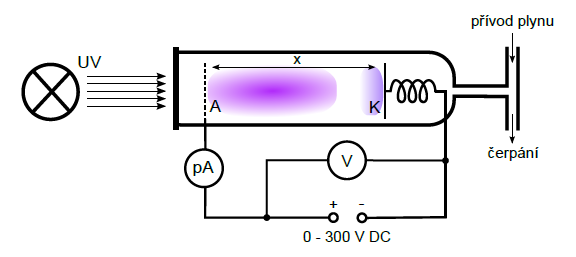
\includegraphics[width=130mm]{aparatura.png}
	\caption{Schéma použité aparatury}
	\label{aparatura}
\end{figure}

Při měření musíme dbát na to, aby ve výbojce nevznikl samostatný výboj, tedy 
měříme pro hodnoty intenzity elektrického pole 80-120\,$\text{V/\,cm}$. Konstantní elektrické pole v jedné sérii měření udržujeme nastavením napětí na zdroji a přizpůsobením vzájemné vzdálenosti elektrod, přičemž posouváme i UV lampou, aby vzdálenost mezi ní a katodou byla stálá. Výstupem z~měření je poloha katody $x$, hodnota napětí $U$ 
a proud $i$ pro několik hodnot konstantní intenzity elektrického pole $E$. Pro 
každou změnu intenzity pole naladíme irisovou clonu UV výbojky tak, abychom 
měli maximální proud okolo 1800\,pA z~důvodu rozsahu na přístroji do 1999\,pA. 
Proud je tedy řádově pA až nA, pro zlepšení přesnosti měření z~ampérmetru 
odečítáme vždy 3~hodnoty a dále budeme pracovat s~jejich průměrem. Tlak je 
konstantní o~hodnotě $p$\,=\,79,5\,Pa.

V~rovnicích (\ref{2}) a (\ref{3}) lze nahradit počet elektronů proudem. 
Z~naměřených dat můžeme sestavit graf závislosti $i = i_0 f(x)$, viz 
obr.~\ref{ifx80-120} a obr.~\ref{ifx90-110}. Body jsou proložené exponenciální funkcí $i = i_0 \e^{\alpha 
x}$, z~toho získané $i_0$ a $\alpha$ jsou uvedené v~levé části 
tabulky~\ref{tab1}.

Dále můžeme vytvořit graf závislosti $\ln i = \ln i_0 + \alpha x$, viz 
obr.~\ref{lni80-120} a obr.~\ref{lni90-110}. Závislost je proložená lineární funkcí $\ln i =\ln i_0 + \alpha x$, 
získané $i_0$ a $\alpha$ jsou uvedené v~pravé části tabulky~\ref{tab1}.

V~obou případech je vidět, že s~rostoucí intenzitou elektrického pole $E$ proud $i_0$ klesá a ionizační koeficient $\alpha$ roste.

\begin{figure}[h!]
	\centering
	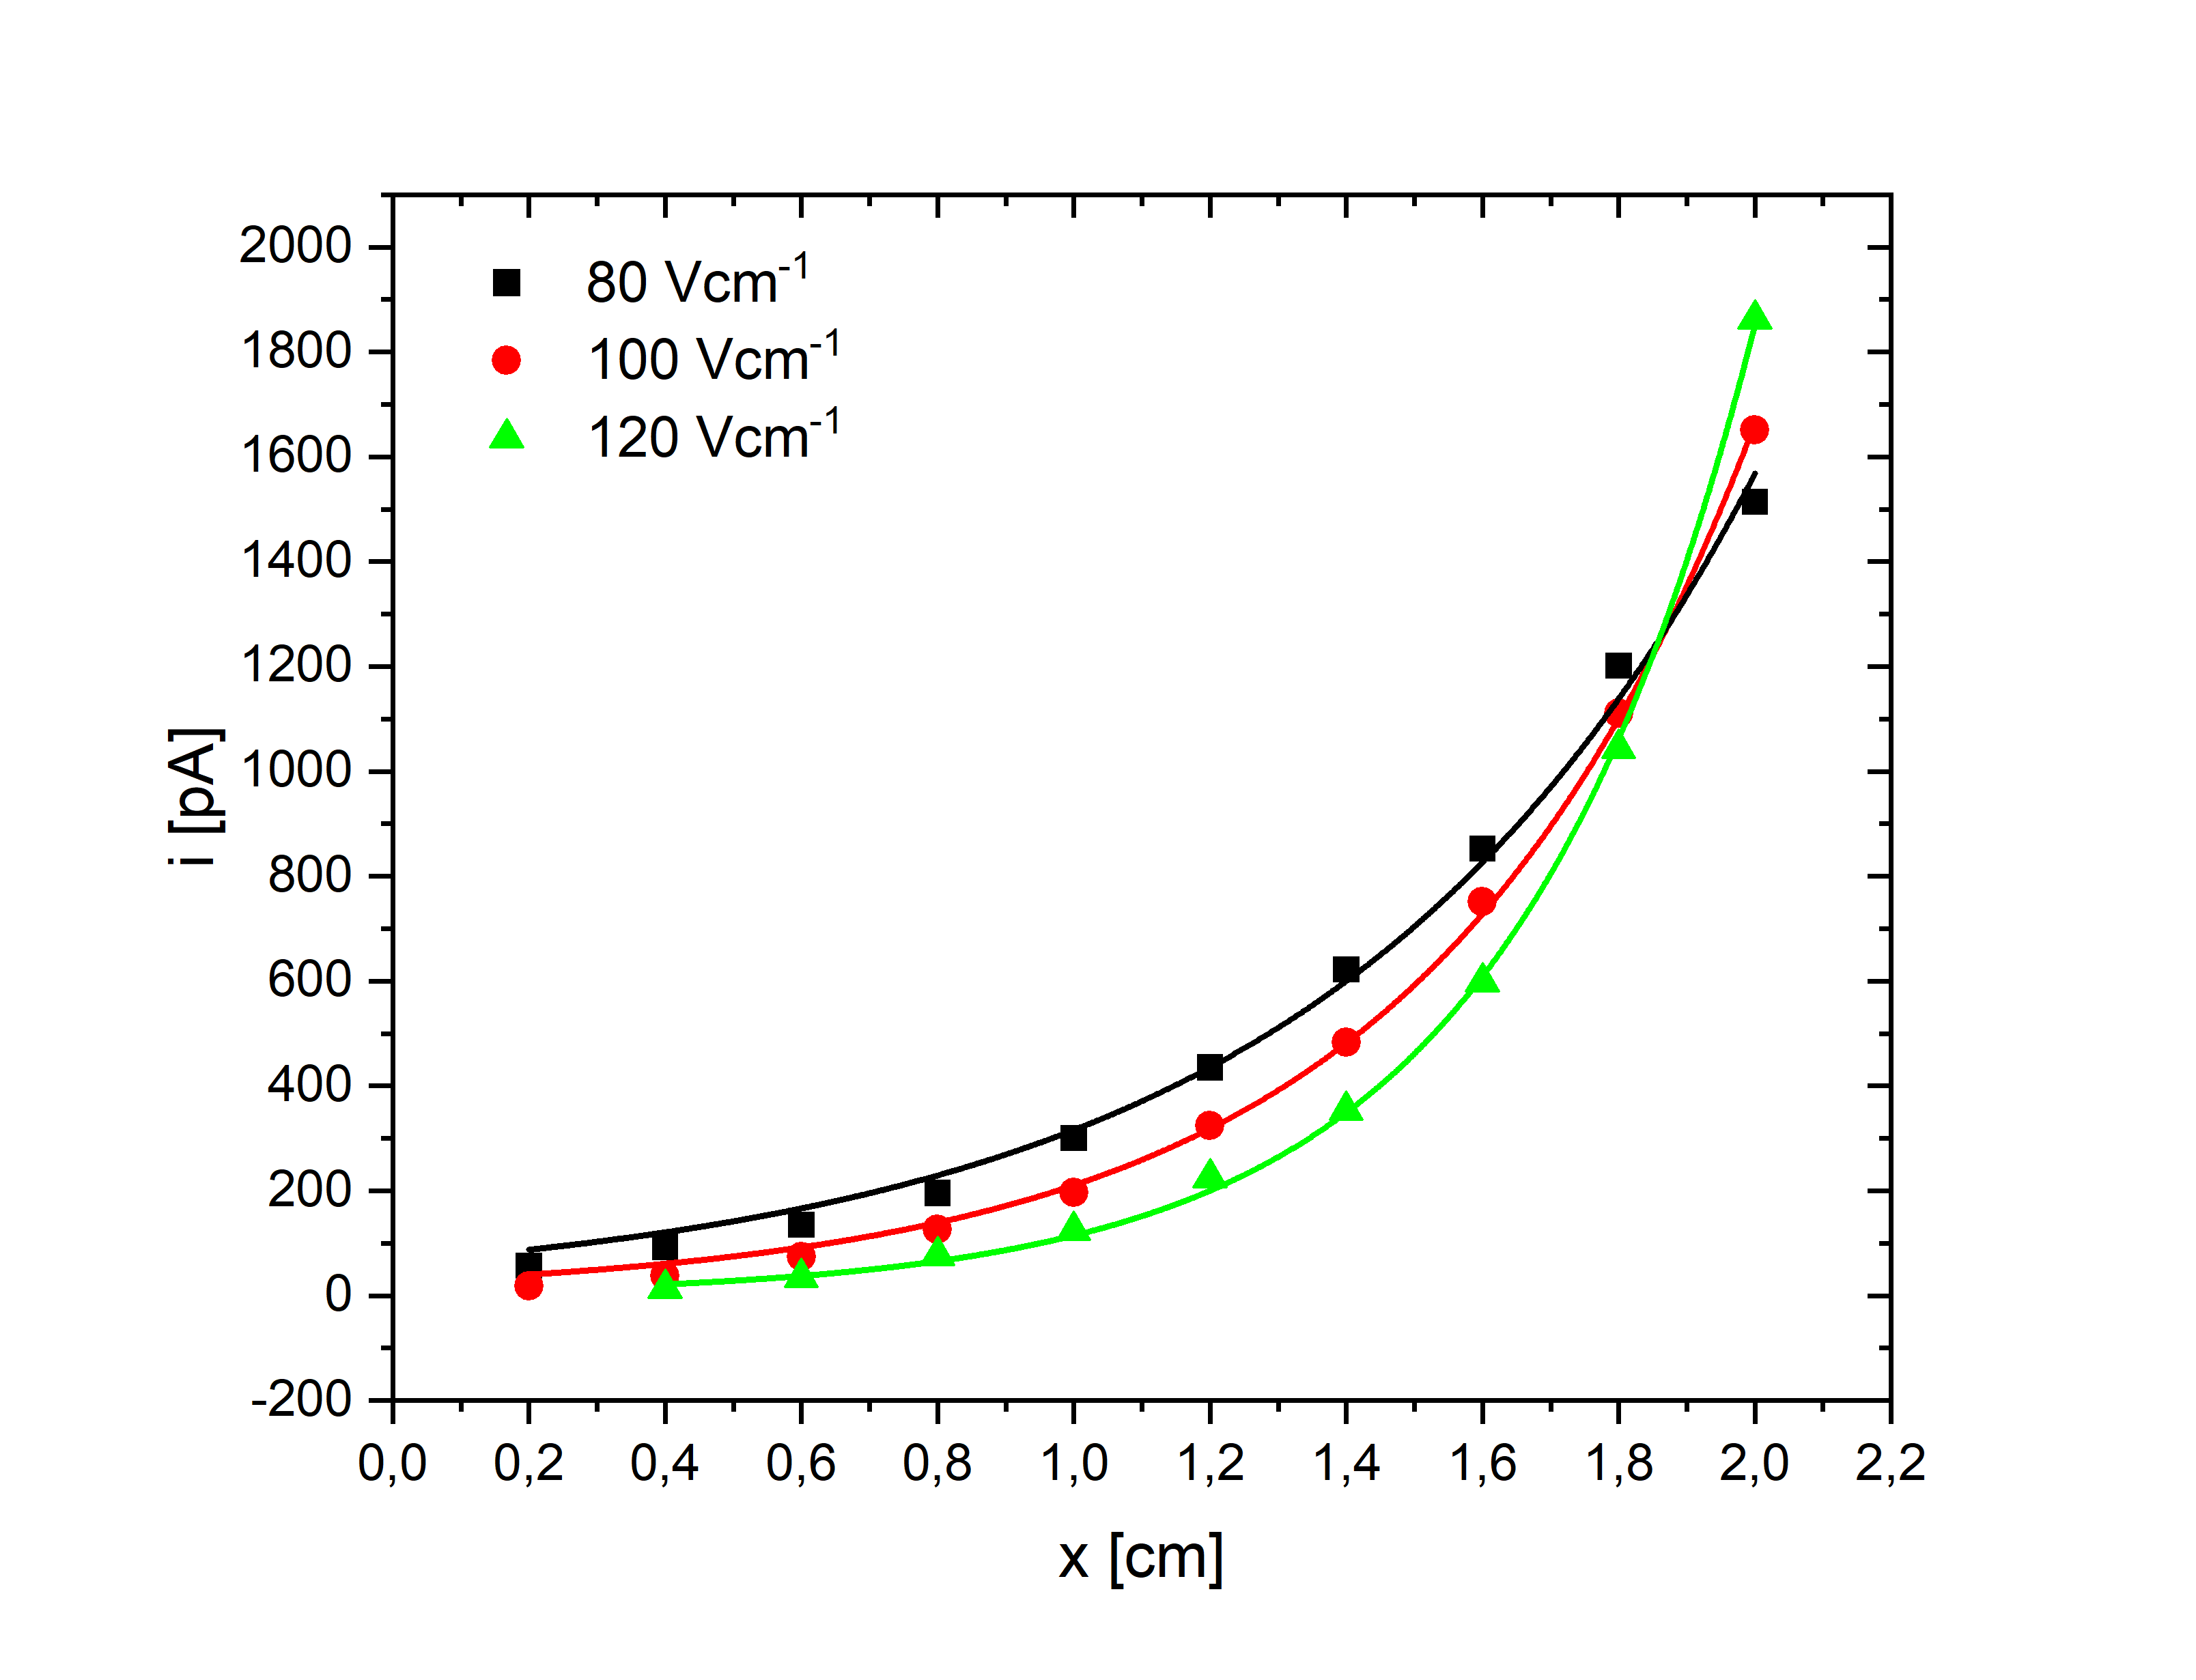
\includegraphics[width=145mm]{ifx80-120.png}
	\caption{Graf závislosti $i$ na $x$.}
	\label{ifx80-120}
\end{figure}

\begin{figure}[h!]
	\centering
	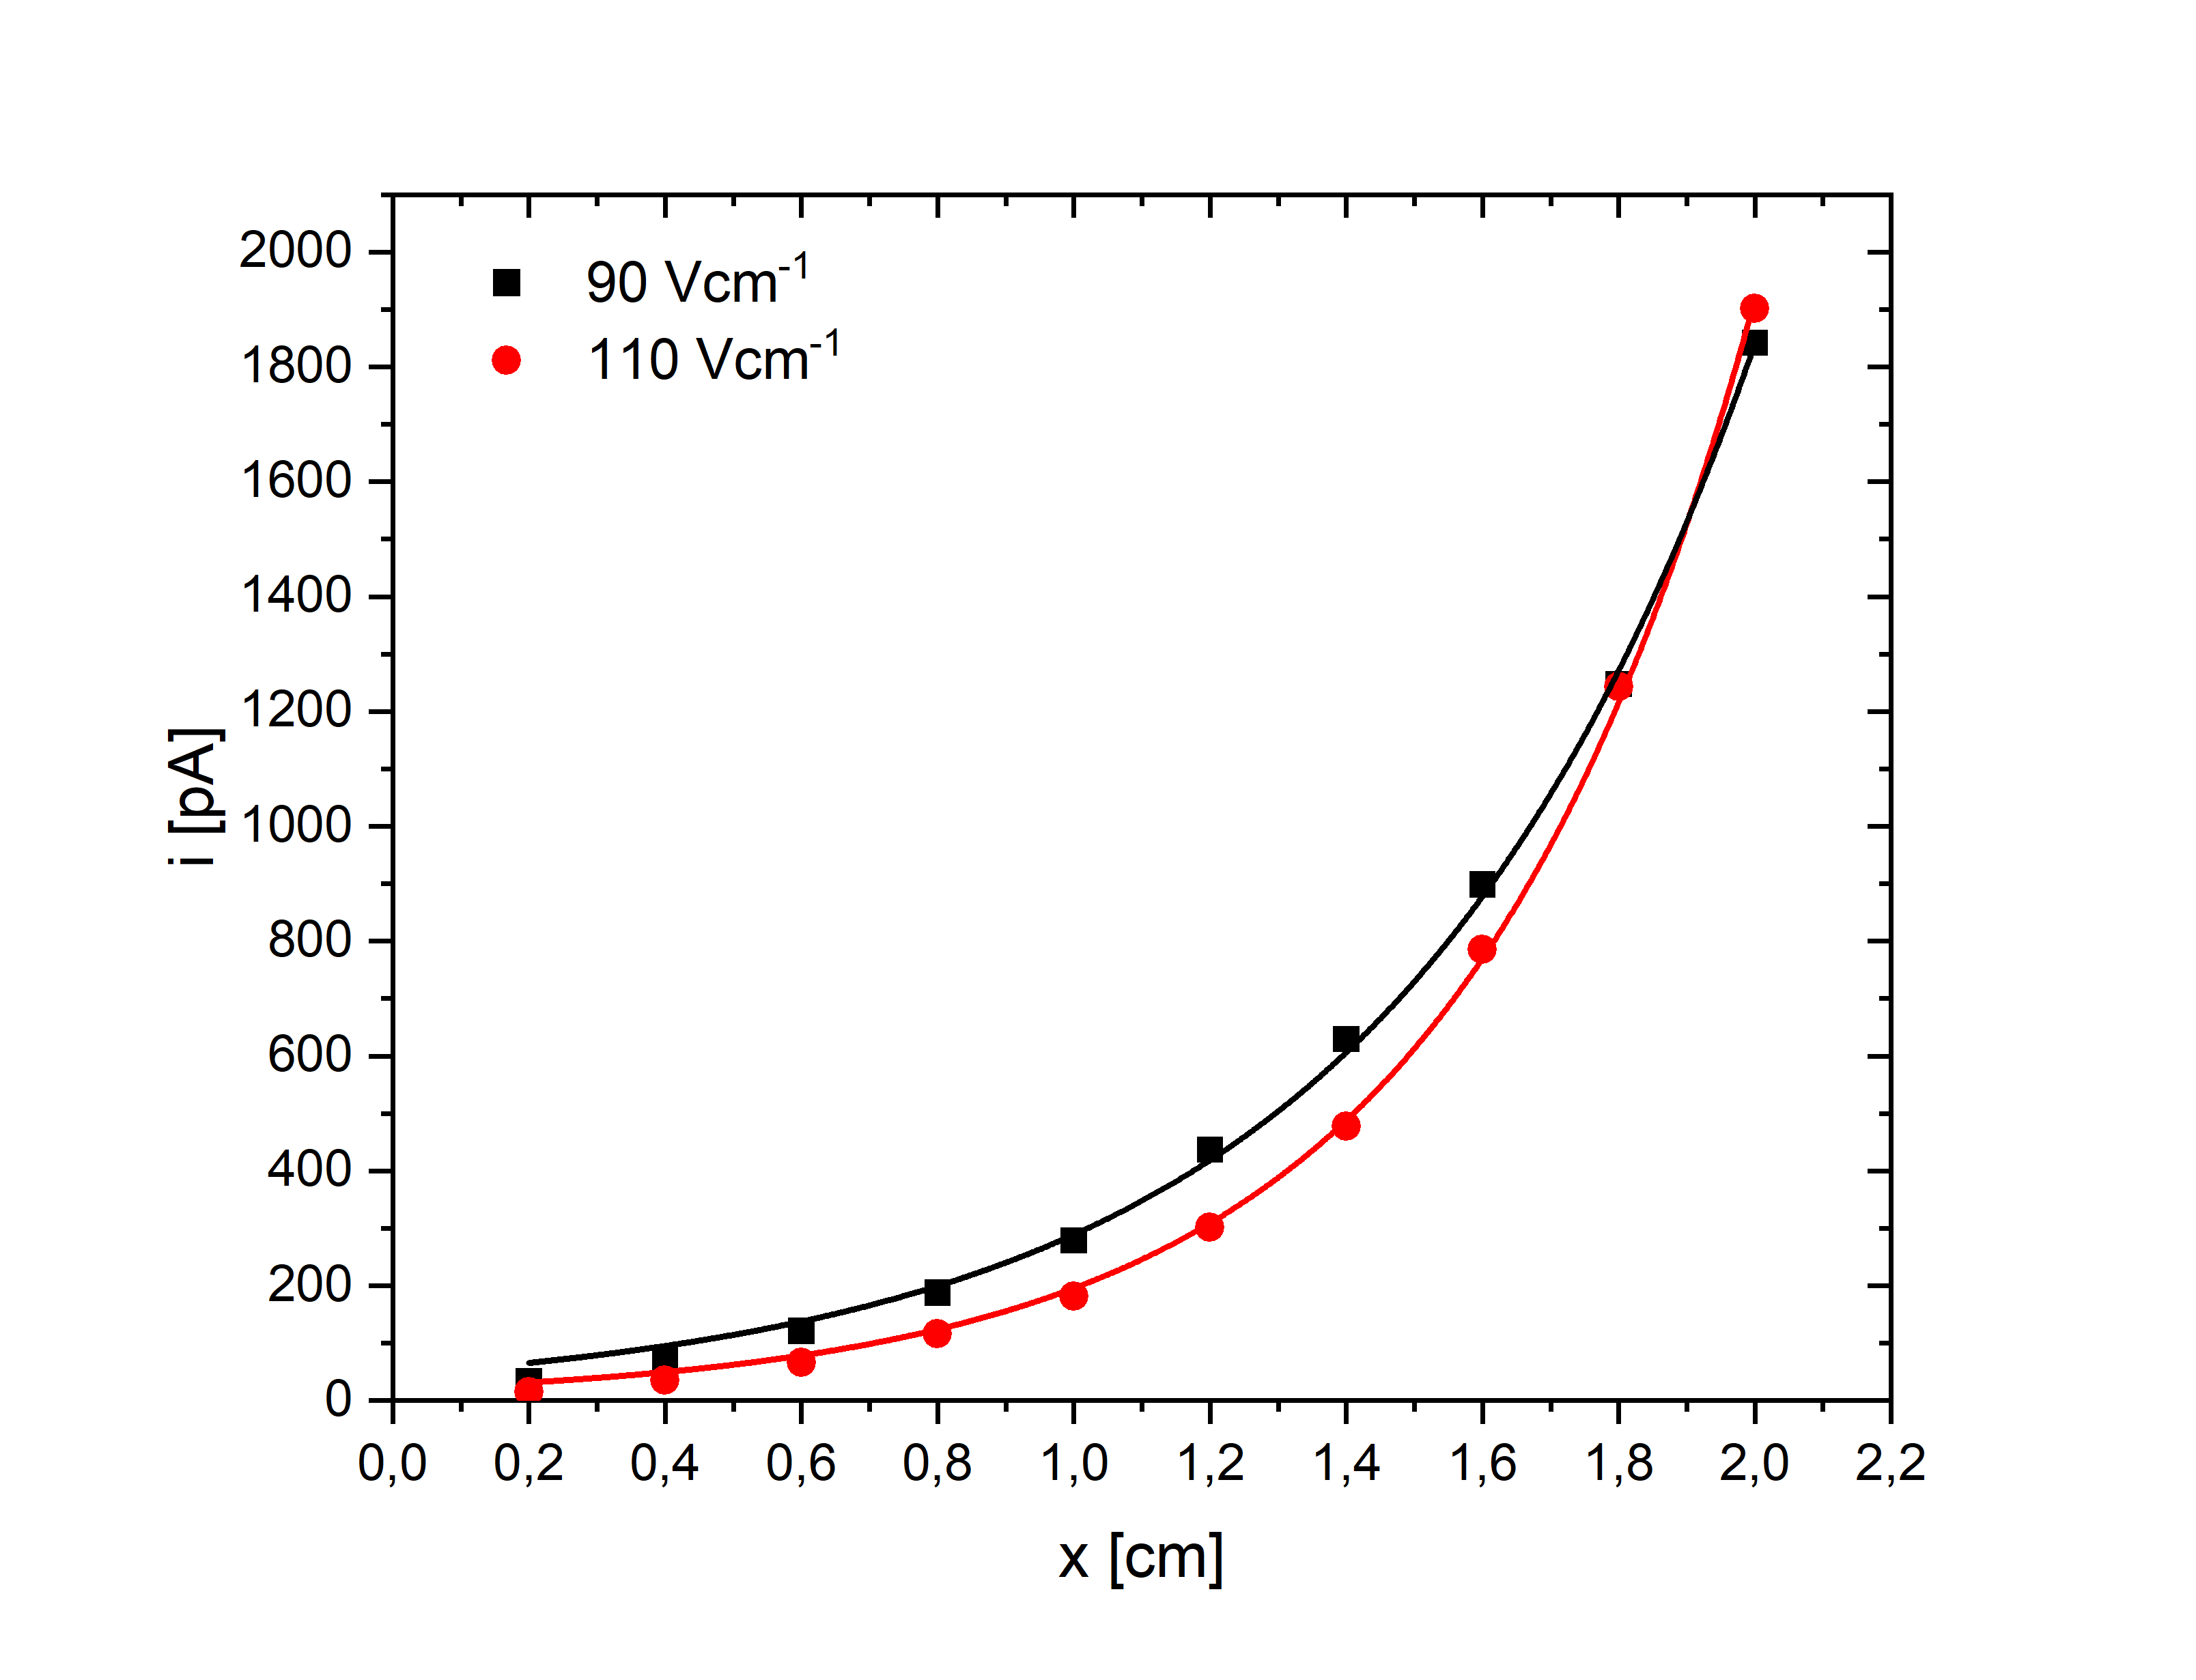
\includegraphics[width=145mm]{ifx90-110.png}
	\caption{Graf závislosti $i$ na $x$.}
	\label{ifx90-110}
\end{figure}


\begin{figure}[h!]
	\centering
	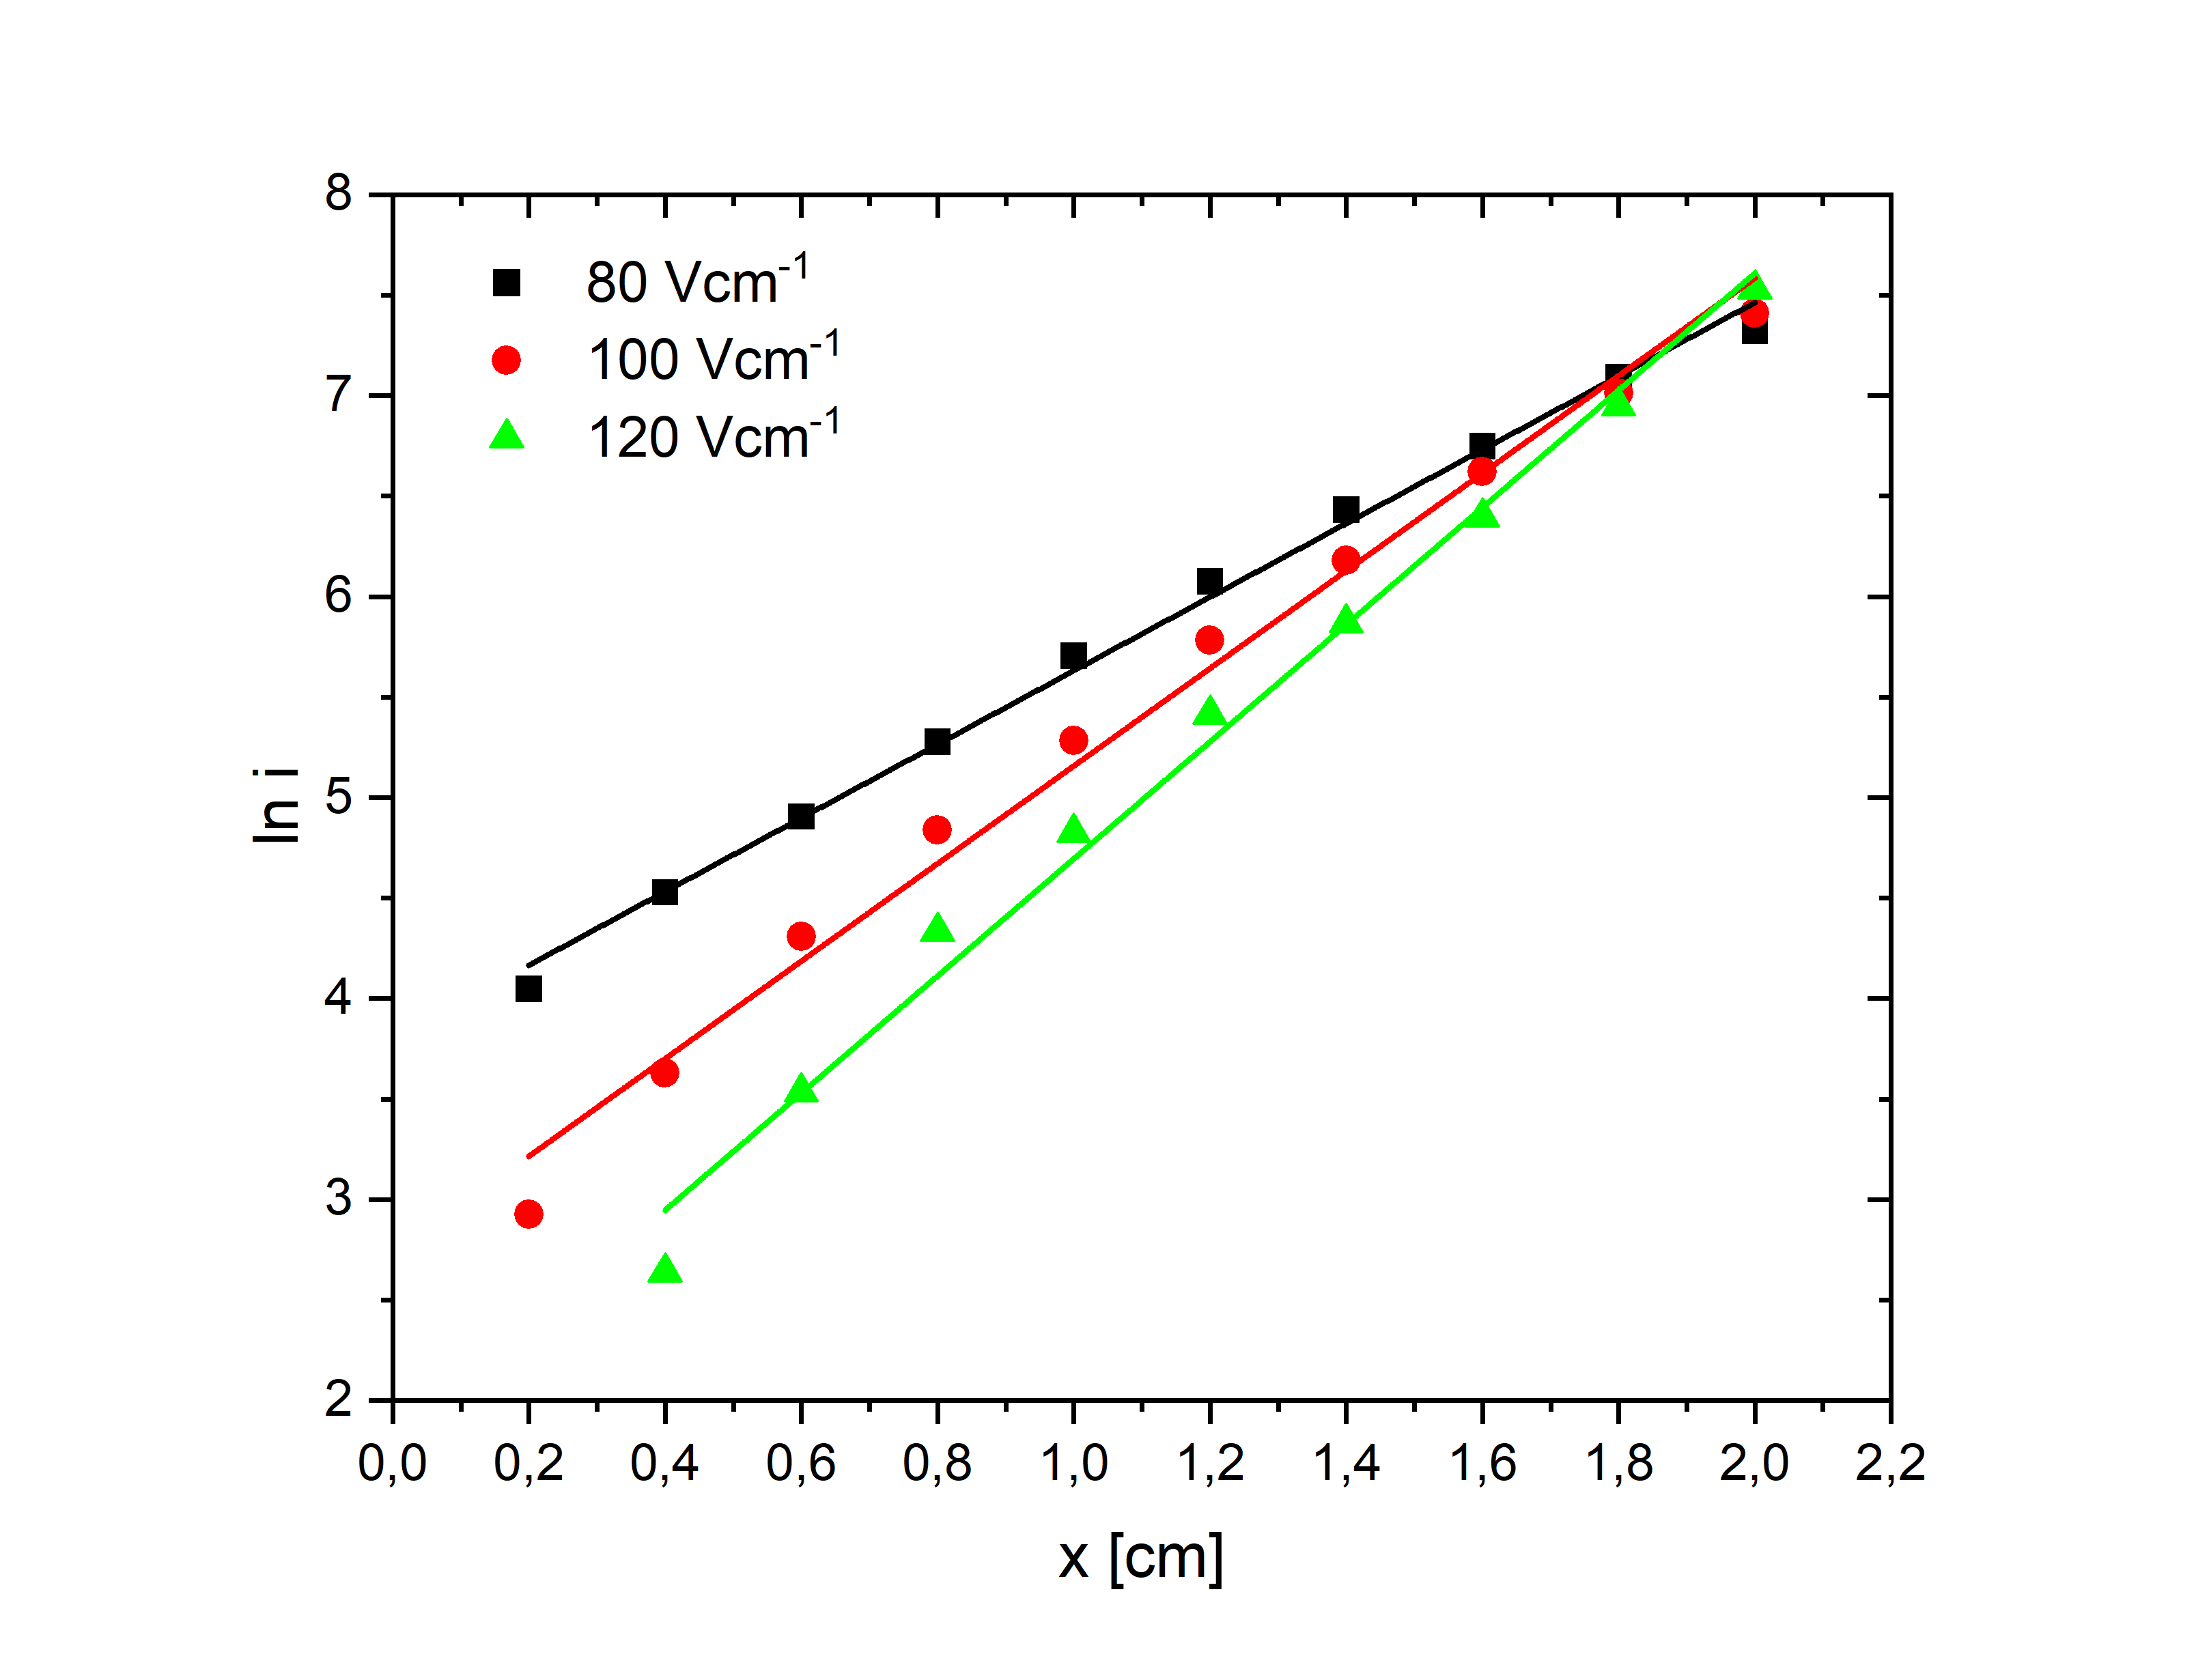
\includegraphics[width=145mm]{lni80-120.png}
	\caption{Graf závislosti $\ln i$ na $x$.}
	\label{lni80-120}
\end{figure}

\begin{figure}[h!]
	\centering
	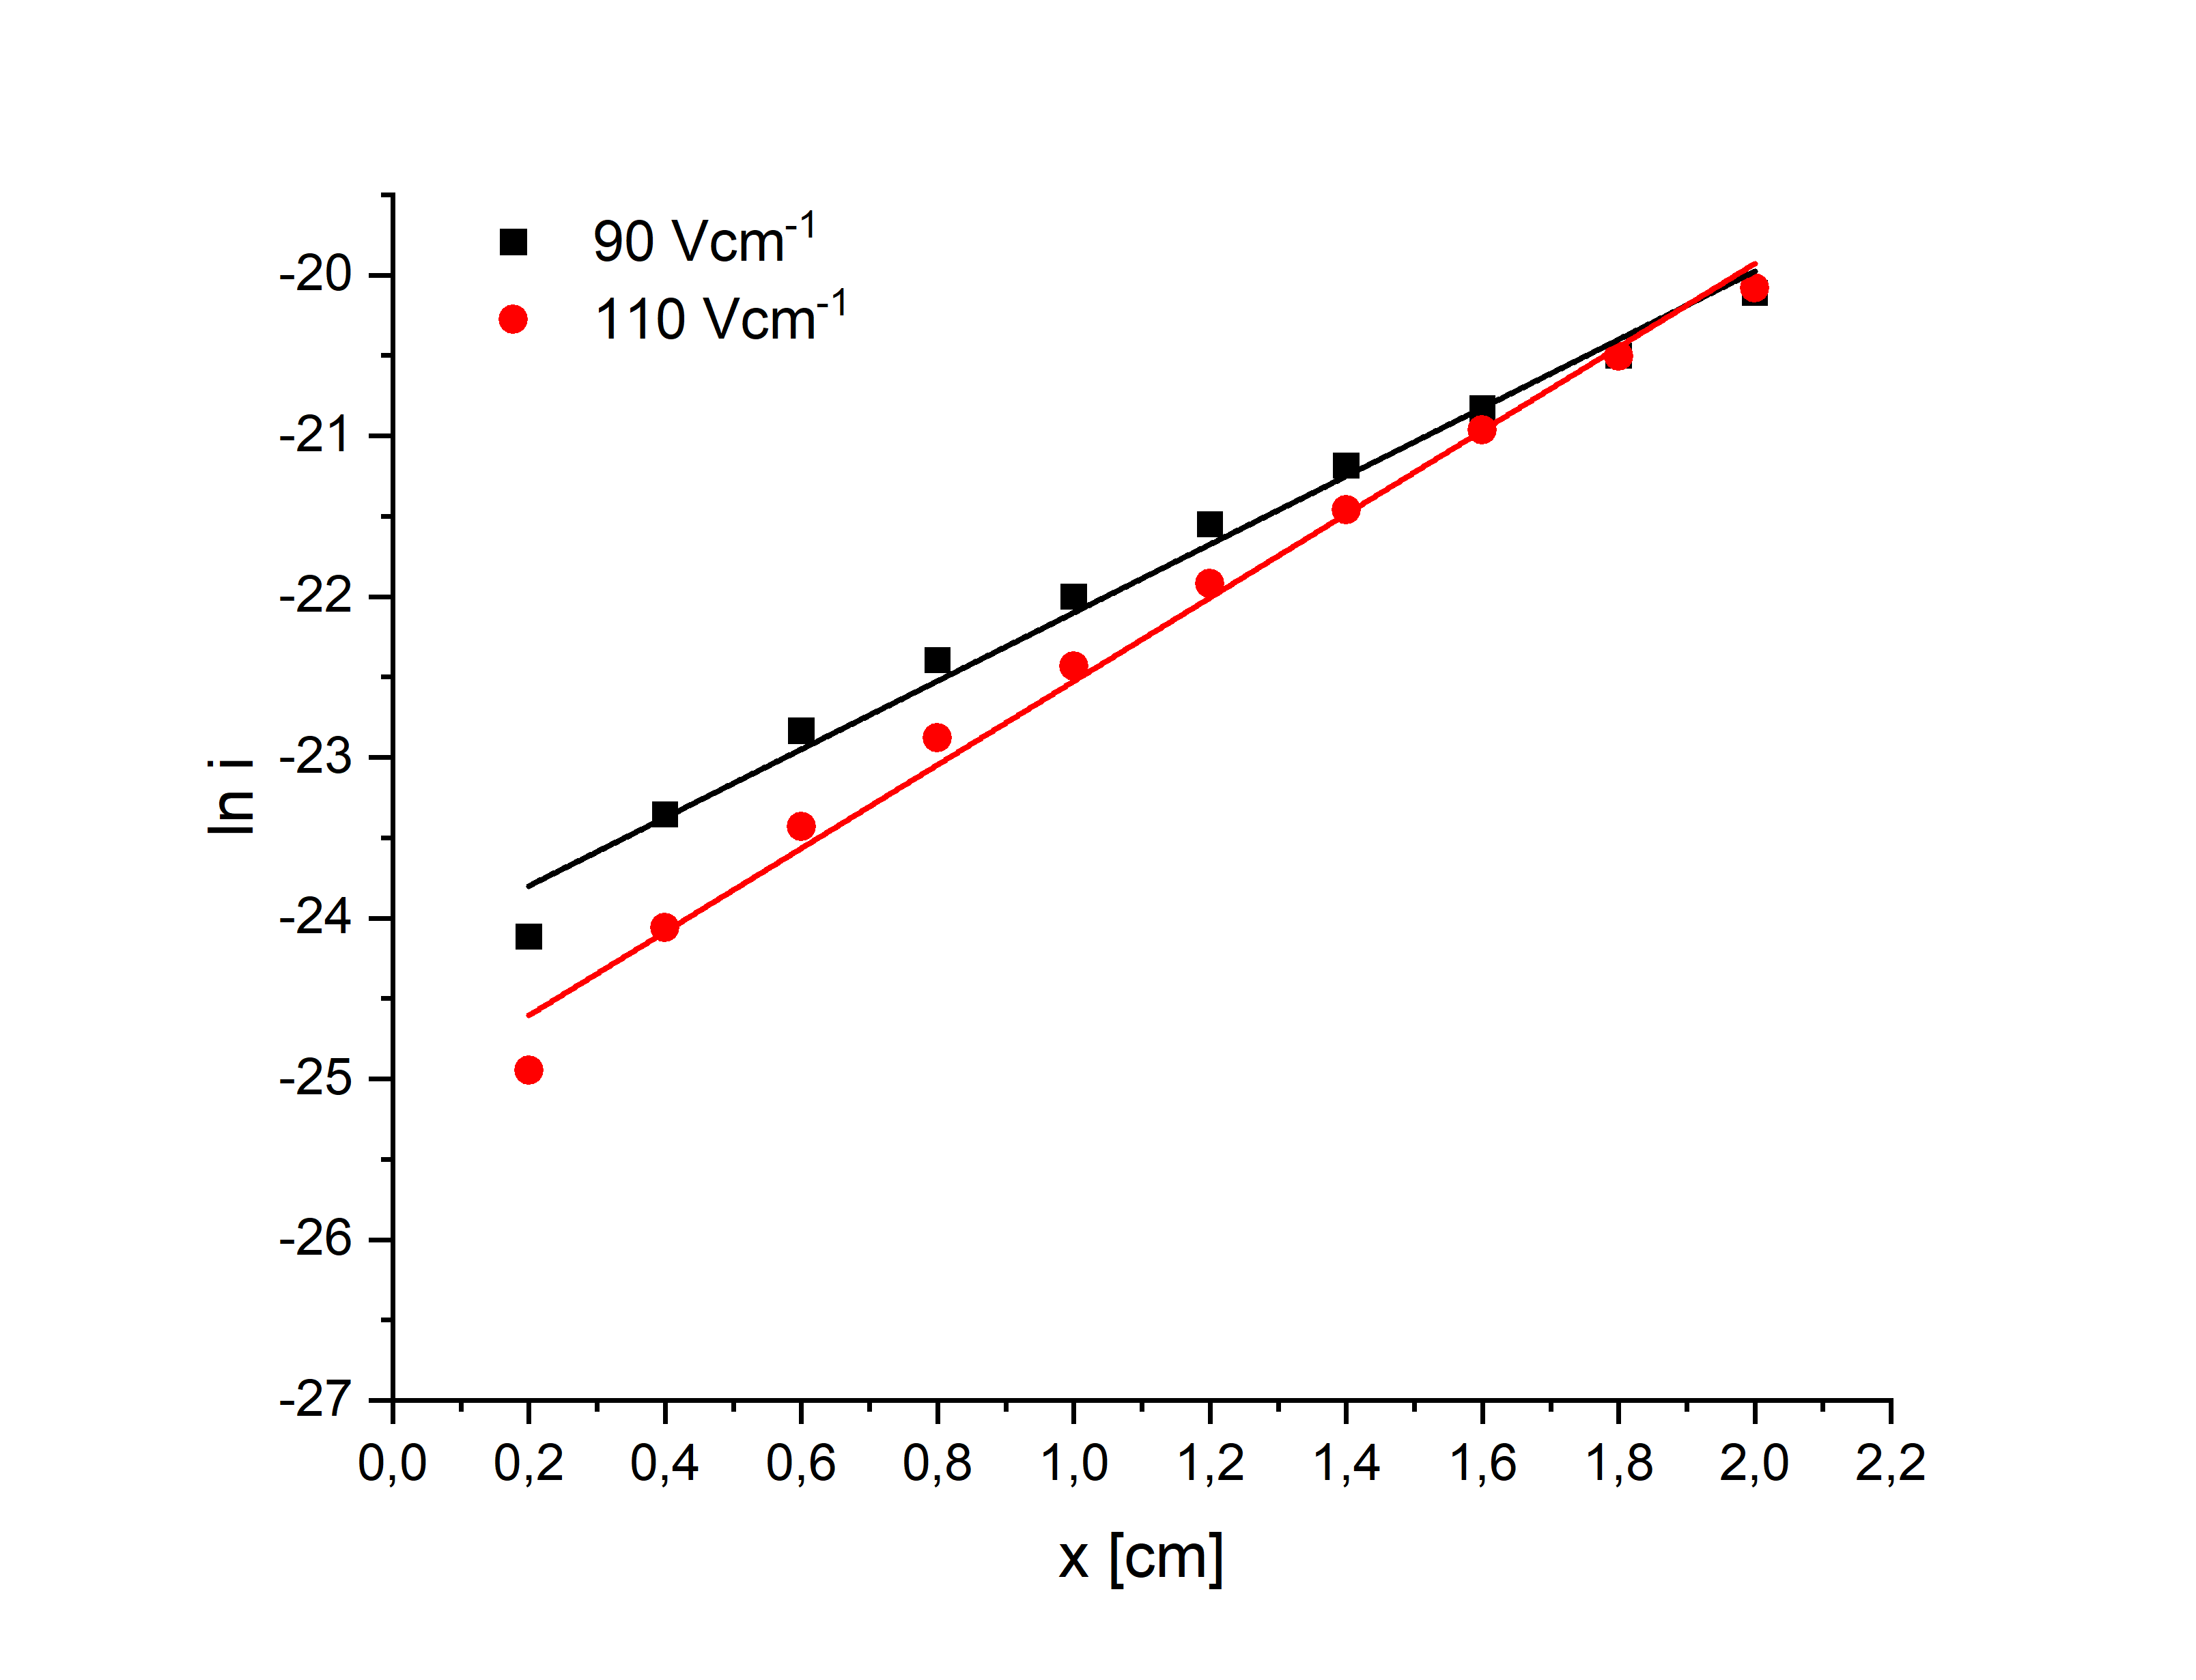
\includegraphics[width=145mm]{lni90-110.png}
	\caption{Graf závislosti $\ln i$ na $x$.}
	\label{lni90-110}
\end{figure}


\begin{center}
	\begin{table}[h]
		\centering
		\caption{Hodnoty proudů $i_0$ a ionizačních koeficientů $\alpha$ pro různé hodnoty $E$.}
		\label{tab1}
		\begin{tabular}{|c|c|c|c|c|} \hline
			\multicolumn{1}{|c|}{}  & \multicolumn{2}{c|}{$i = i_0 \e^{\alpha 
			x}$}& \multicolumn{2}{c|}{$\ln i = \ln i_0 + \alpha x$}  \\ \hline
			$E$ [Vcm$^{-1}$] & $i_0$ [pA] & $\alpha$ [cm$^{-1}$] & $i_0$ [pA] & $\alpha$ [cm$^{-1}$] \\ \hline
			80 & 63,7 $\pm$ 6,6 & 1,60 $\pm$ 0,06 & 44,7 $\pm$ 1,1 & 1,83 $\pm$ 
			0,04\\ \hline
			90 & 45,3 $\pm$ 2,8 & 1,85 $\pm$ 0,03& 30,2 $\pm$ 1,1 & 2,12 $\pm$ 
			0,08\\ \hline
			100 & 26,7 $\pm$ 1,7 & 2,07 $\pm$ 0,03 & 15,3 $\pm$ 1,1 & 2,43 
			$\pm$ 0,09\\ \hline
			110 & 19,9 $\pm$ 1,2 & 2,23 $\pm$ 0,03 & 12,3 $\pm$ 1,1 & 2,60 
			$\pm$ 0,09 \\ \hline
			120 & 7,1 $\pm$ 0,5 & 2,80 $\pm$ 0,04 & 5,9 $\pm$ 1,2 & 2,91 
			$\pm$ 0,11 \\ \hline
			
		\end{tabular}
	\end{table}
\end{center}

%\begin{center}
%	\begin{table}[h]
%		\centering
%		\caption{Hodnoty proudů $i_0$ a ionizačních koeficientů $\alpha$ pro 
%různé hodnoty $E$.}
%		\label{tab1}
%		\begin{tabular}{|c|c|c|c|c|} \hline
%			\multicolumn{1}{|c|}{}  & \multicolumn{2}{c|}{$i = i_0 \e^{\alpha 
%					x}$}& \multicolumn{2}{c|}{$i = i_0 + \alpha x$}  \\ \hline
%			$E$ [Vcm$^{-1}$] & $i_0$ [pA] & $\alpha$ [cm$^{-1}$] & $i_0$ [pA] & 
%$\alpha$ [cm$^{-1}$] \\ \hline
%			80 & 63,65 $\pm$ 6,62 & 1,60 $\pm$ 0,06 & 44,65 $\pm$ 1,06 & 1,83 
%$\pm$ 0,04\\ \hline
%			90 & 45,30 $\pm$ 2,79 & 1,85 $\pm$ 0,03& 30,15 $\pm$ 1,11 & 2,12 
%$\pm$ 0,08\\ \hline
%			100 & 26,65 $\pm$ 1,70 & 2,07 $\pm$ 0,03 & 15,32 $\pm$ 1,12 & 2,43 
%$\pm$ 0,09\\ \hline
%			110 & 19,92 $\pm$ 1,23 & 2,23 $\pm$ 0,03 & 12,25 $\pm$ 1,12 & 2,60 
%$\pm$ 0,09 \\ \hline
%			120 & 7,09 $\pm$ 0,48 & 2,80 $\pm$ 0,03 & 3,73 $\pm$ 1,28 & 3,23 
%$\pm$ 0,20 \\ \hline
%			
%		\end{tabular}
%	\end{table}
%\end{center}

\newpage
Jelikož jsme provedli měření pro několik hodnot $E/\,p$, můžeme sestavit grafy 
závislosti $\ln \alpha/\,p = f(p/\,E)$ a proložit jej lineární funkcí $\ln \alpha/\,p 
= \ln A~- \frac{Bp}{E}$, která vychází z~úpravy rovnice~(\ref{5}). To provedeme 
jak pro $\alpha$ získané z~exponenciálního fitu, tak i pro $\alpha$ z~lineárního fitu. Následně pomocí rovnice~(\ref{6}) určíme ionizační potenciál 
argonu $U_\text{i}$, viz tab.~\ref{tab2}. Tabulková hodnota pro argon je $U_\text{i} = 
15,76$\,eV. Té se více přiblížil potenciál $U_\text{i}$ = (15,3 $\pm$  1,9)\,eV 
získaný po 
dosazení $\alpha$ z~lineárního fitu.
 
 \begin{figure}[h]
 	\centering
 	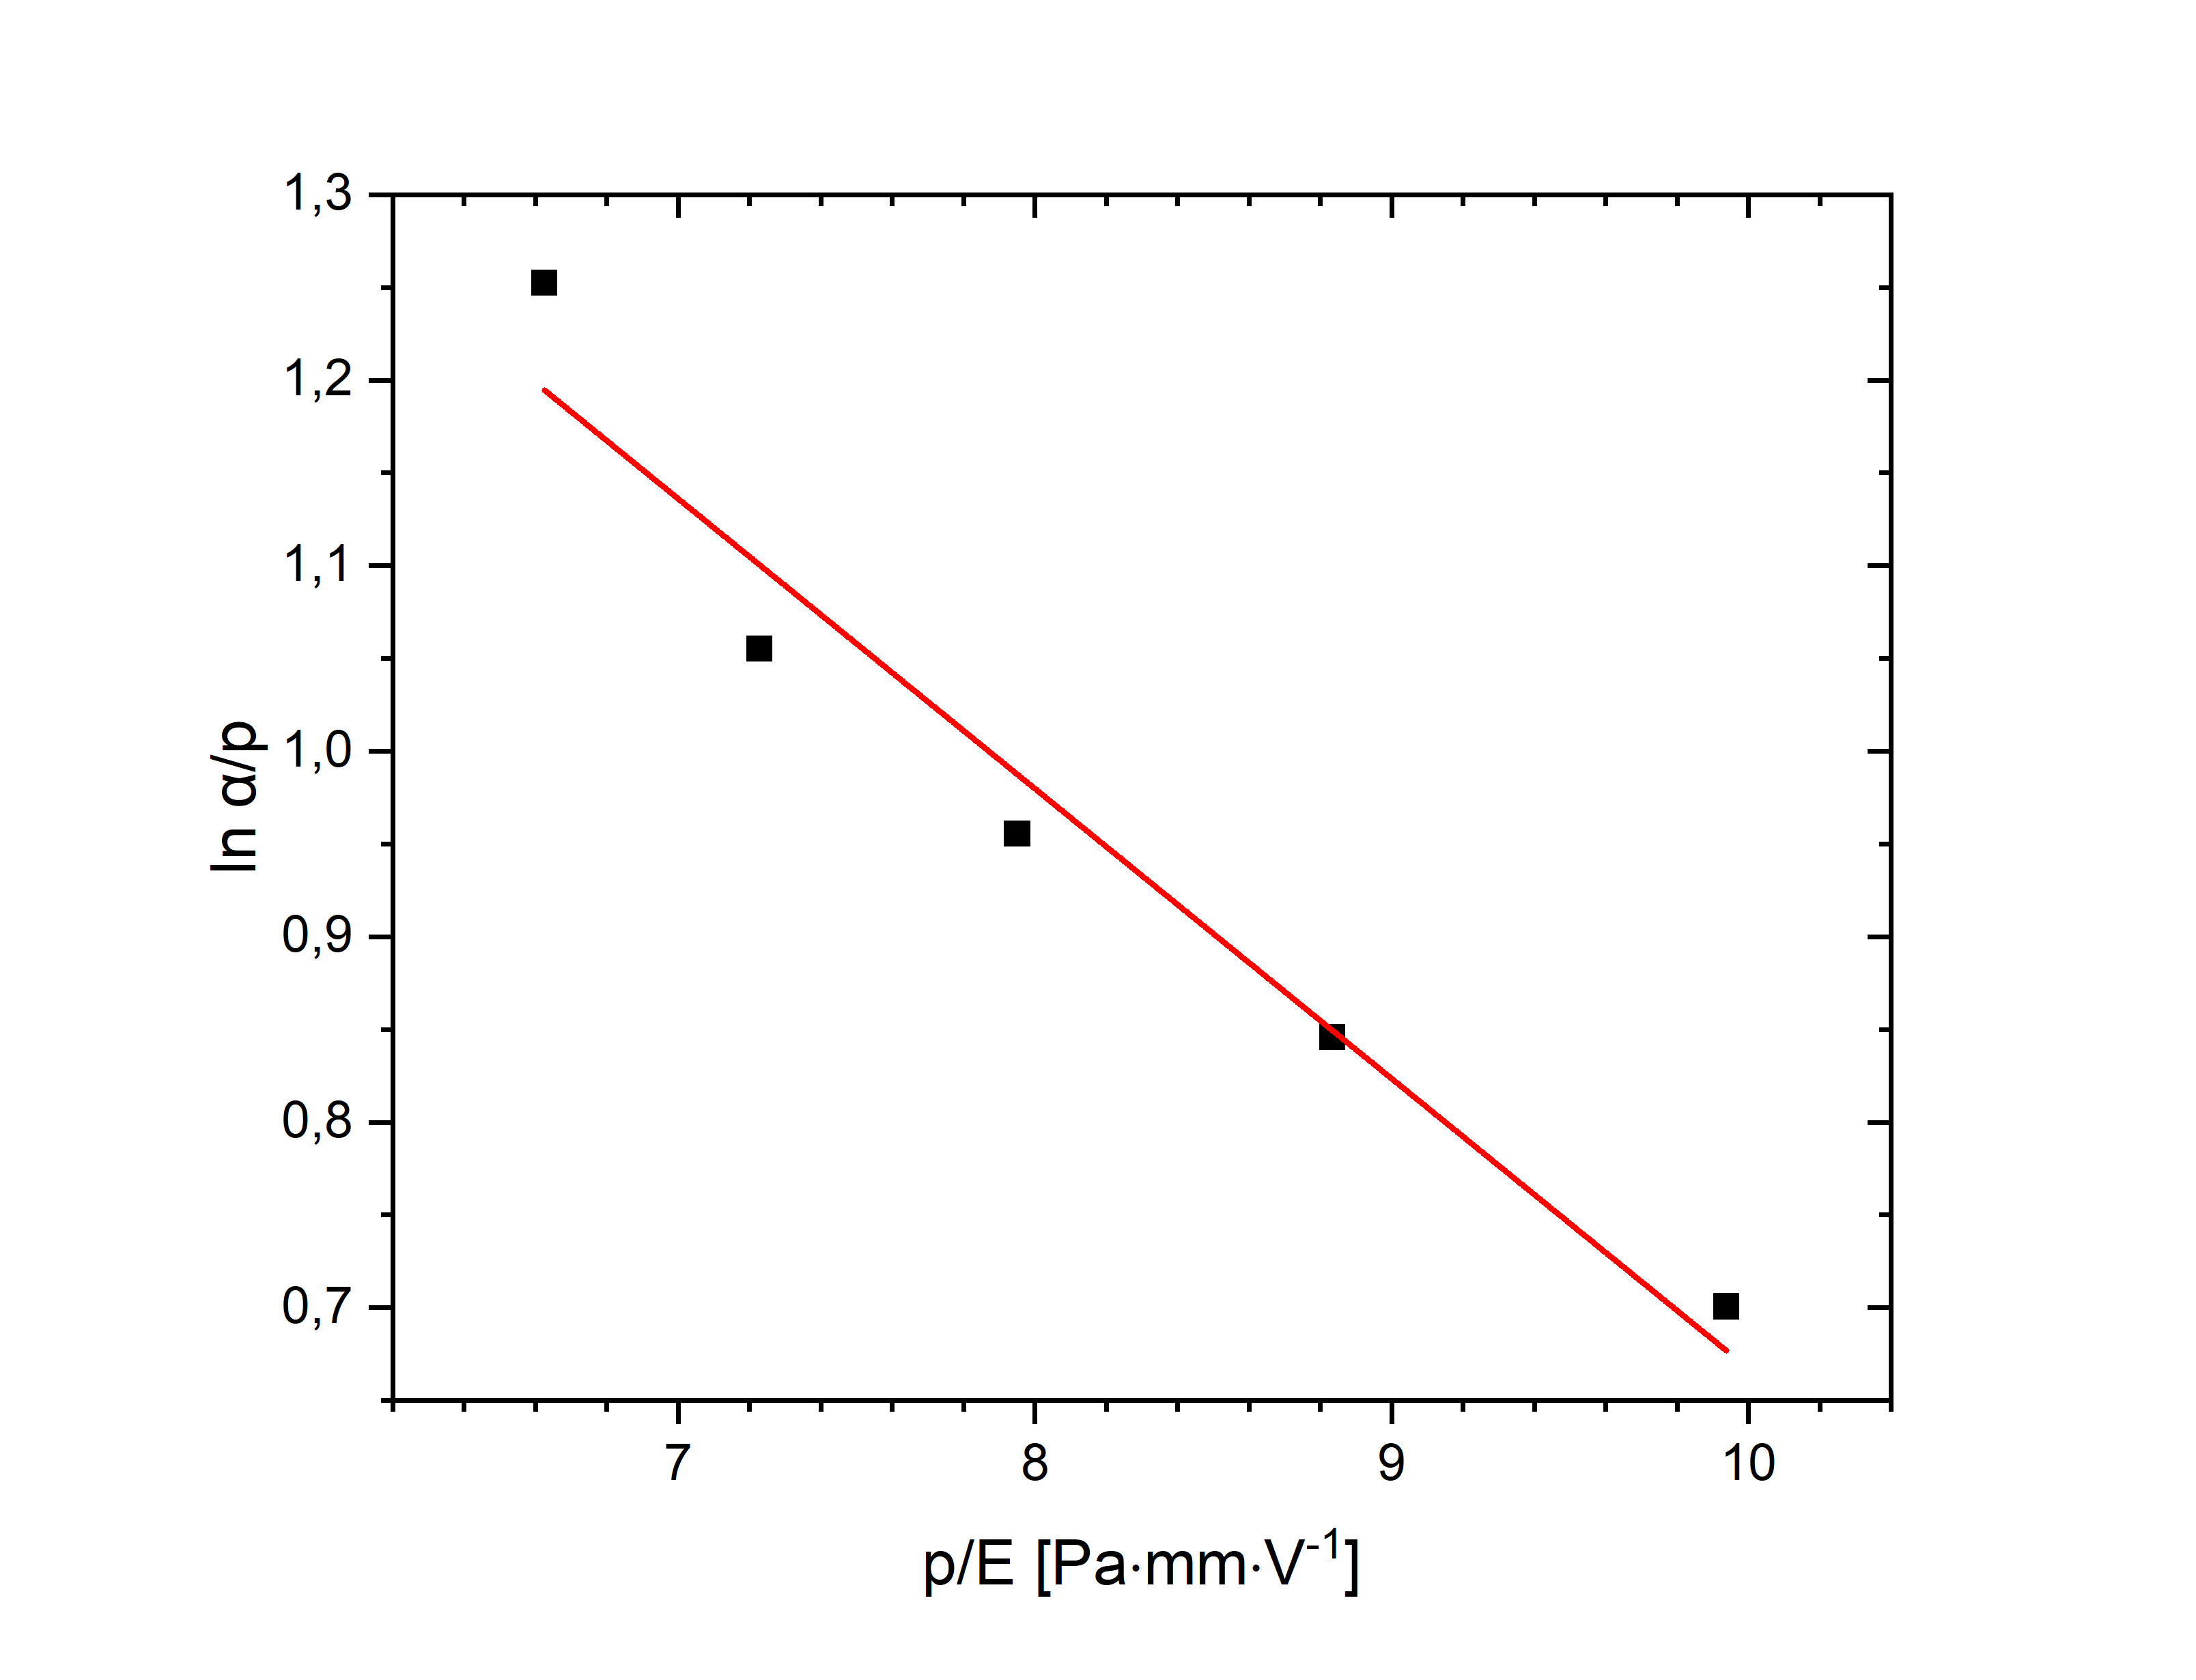
\includegraphics[width=145mm]{exp.png}
 	\caption{Graf závislosti $\ln \alpha/\,p$ na $p/\,E$ pro $\alpha$ 
 	z~exponenciálního fitu.}
 	\label{exp}
 \end{figure}

 \begin{figure}[h]
	\centering
	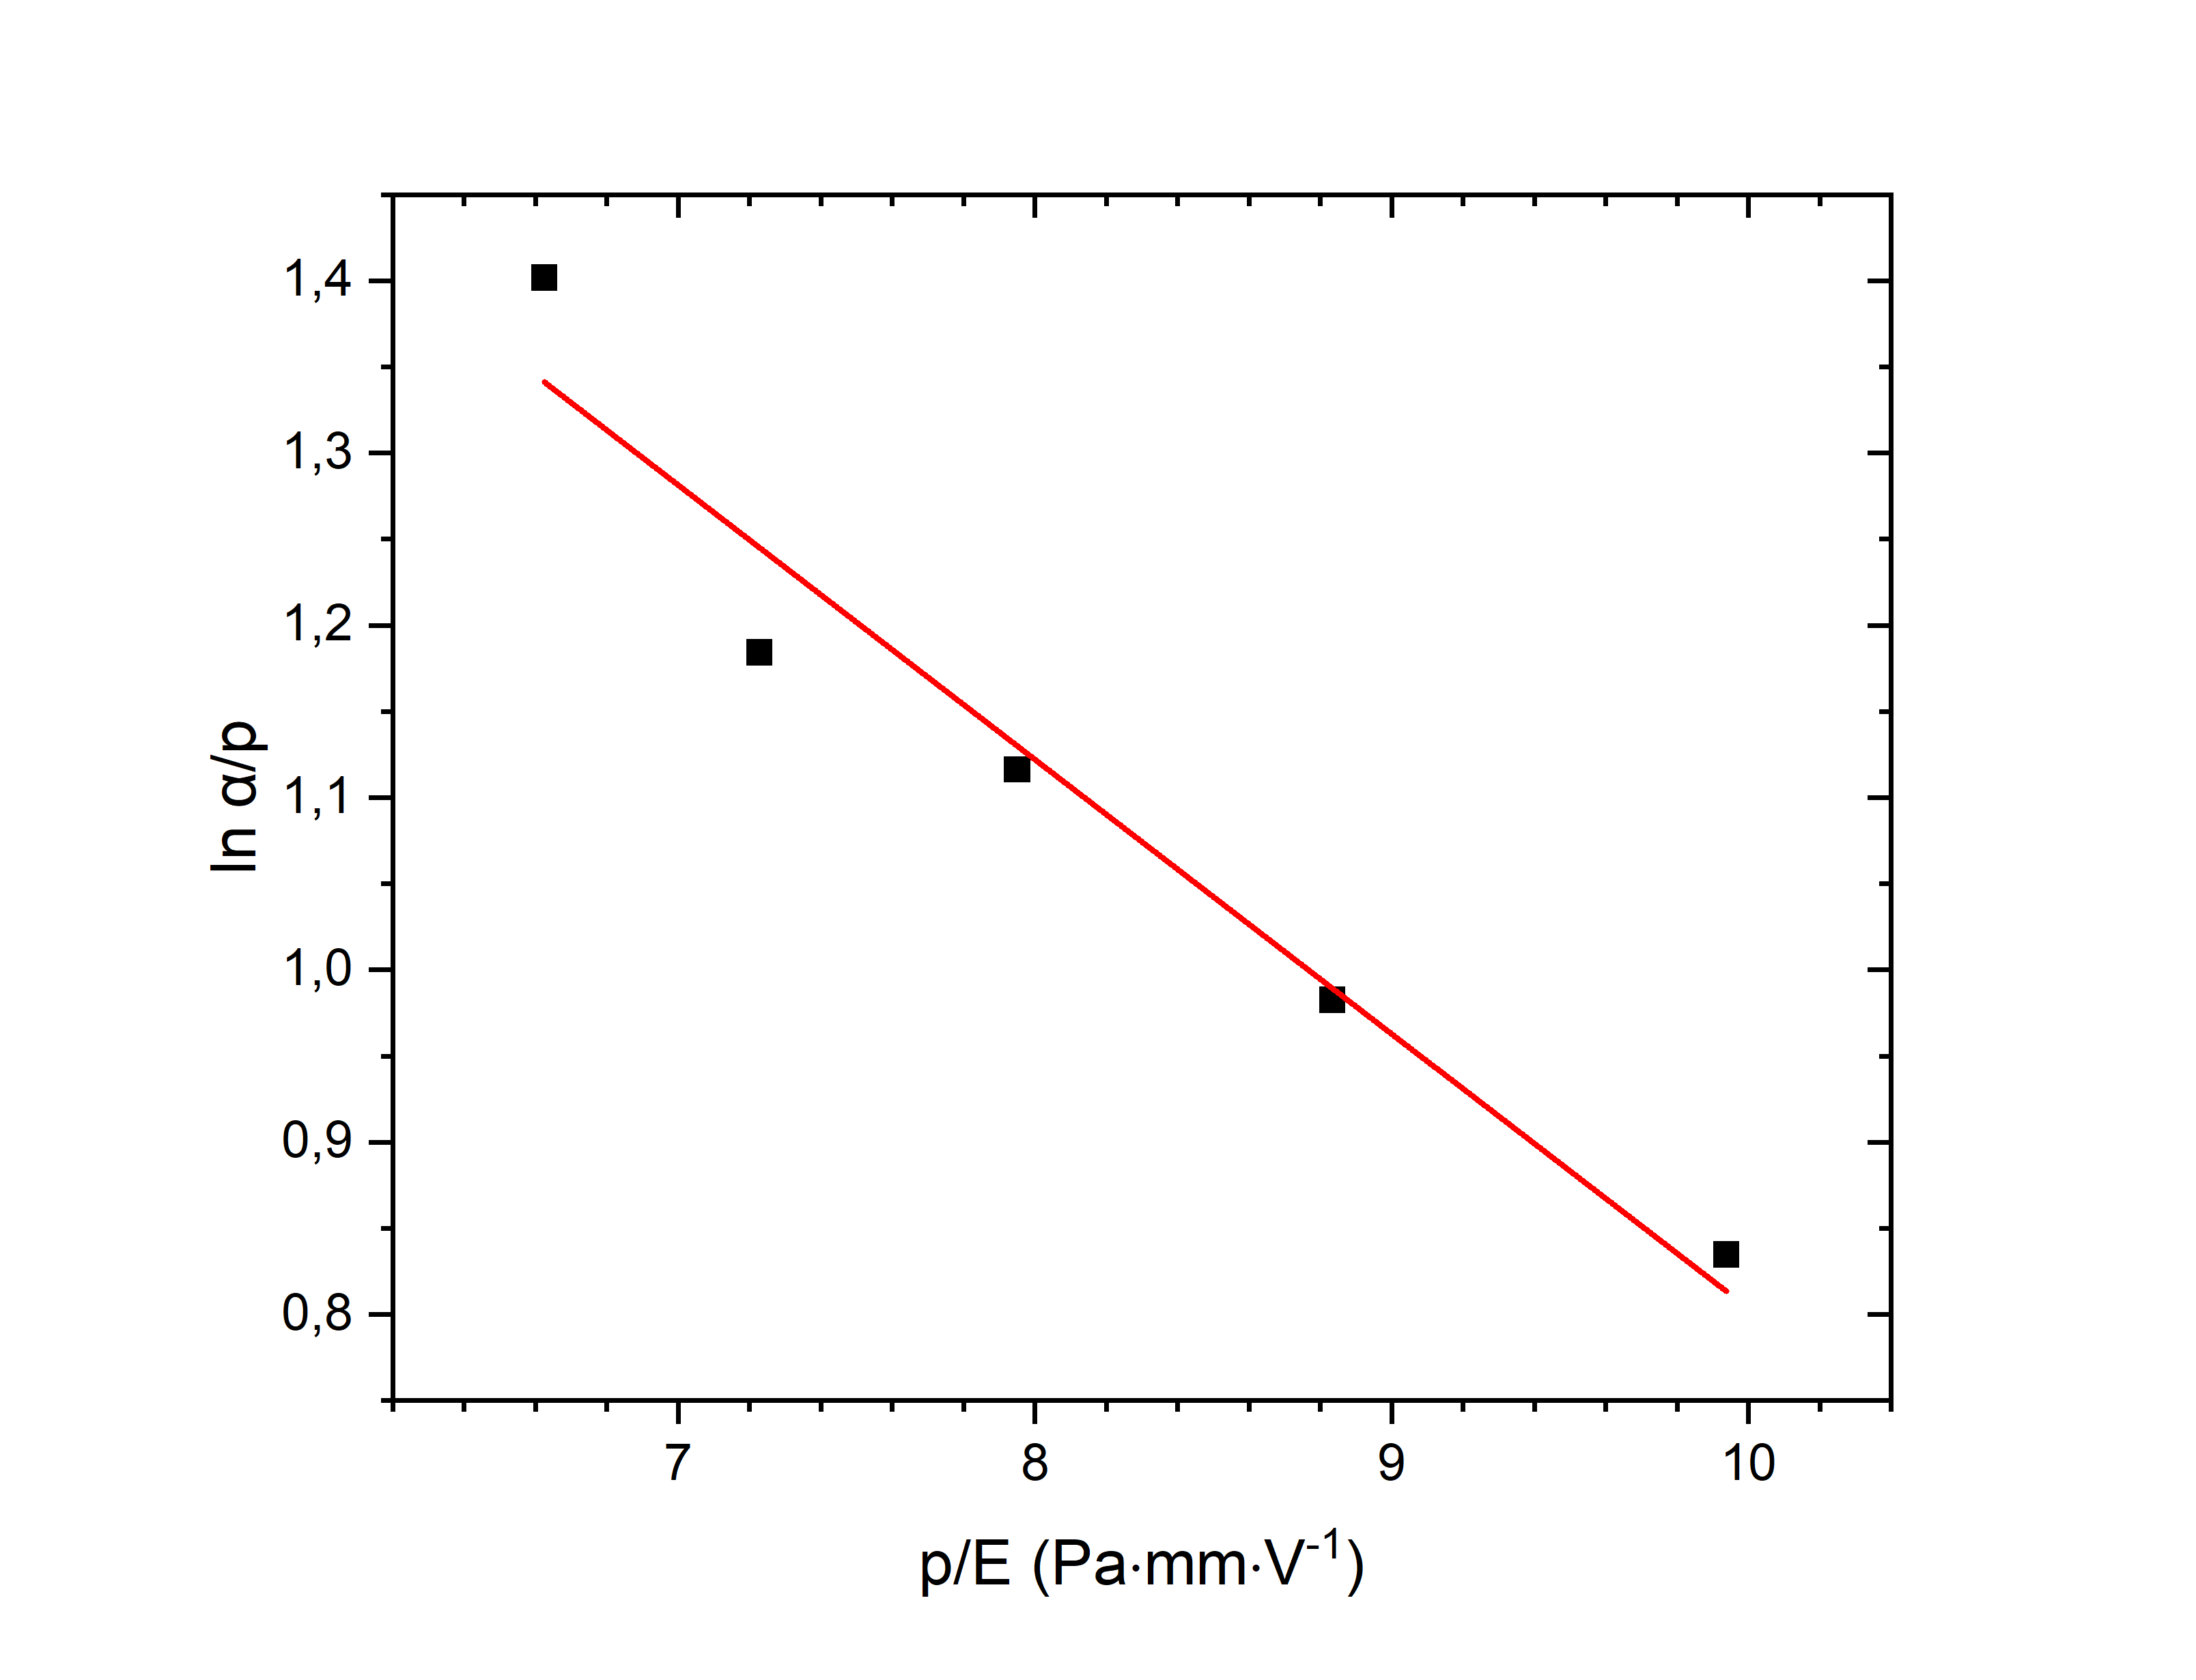
\includegraphics[width=145mm]{lin.png}
	\caption{Graf závislosti $\ln \alpha/\,p$ na $p/\,E$ pro $\alpha$ z~lineárního 
	fitu.}
	\label{lin}
\end{figure}
 
\begin{center}
	\begin{table}[h]
		\centering
		\caption{Hodnoty konstant $A$, $B$ a ionizačních potenciálů $U_\text{i}$ 
		argonu z~$\ln \alpha/\,p = \ln A~- \frac{Bp}{E}$.}
		\label{tab2}
		\begin{tabular}{|c|c|c|c|c|c|} \hline
			\multicolumn{3}{|c|}{Dosazení $\alpha$ z~exponenciálního fitu} & \multicolumn{3}{c|}{Dosazení $\alpha$ z~lineárního fitu}  \\ \hline
			$A$ [\si{\per\pascal\per\meter}] & $B$ [\si{\volt\per\pascal\per\meter}] & $U_\text{i}$ [eV] & $A$ [\si{\per\pascal\per\meter}] & $B$ [\si{\volt\per\pascal\per\meter}] & $U_\text{i}$ [eV] \\ \hline
			9,3 $\pm$ 1,2 & 156 $\pm$ 18 &  16,8 $\pm$ 2,9  & 9,0 $\pm$ 1,0 & 
			137 $\pm$ 5 & 15,3 $\pm$ 1,9\\ \hline
%9,31 $\pm$ 1,16
%156,40 $\pm$ 18,48
%16,80 $\pm$ 2,89	
%10,99 $\pm$ 1,18
%159,31 $\pm$ 19,80	
%14,50 $\pm$ 2,38	
		\end{tabular}
	\end{table}
\end{center}

\newpage
\section{Závěr}
Cílem této úlohy bylo seznámit se s~Townsendovou teorií lavin. Z~měření jsme 
ověřili exponenciální růst proudu s~rostoucí vzdáleností elektrod. Také jsme 
určili první Townsendův koeficient pro různé hodnoty intenzity elektrického 
pole, který roste s~rostoucí $E$. Nakonec jsme získali ionizační potenciál 
argonu ze závislostí $i = f(x)$ a $\ln i = f(x)$, který nám vyšel přesněji
z~lineárního proložení $\ln i = f(x)$ jako $U_\text{i}$ = (15,3 $\pm$  1,9)\,eV, 
tabulková hodnota je $U_\text{i} = 15,76$\,eV. V~případě fitu exponenciální závislosti metodou nejmenších čtverců mají body o~vyšší y hodnotě ve fitu větší váhu než ty při nižších y. 


\end{document}
